\documentclass[12pt]{book}
\usepackage[utf8]{inputenc}
\usepackage[margin=1.25in]{geometry}
\usepackage{graphicx}
\usepackage{amsmath , amssymb}
\usepackage{bm}
\usepackage{esvect}
\usepackage{centernot}

\begin{document}
    \chapter{Rappel des lois de la mecanique Newtonienne}
        \section{Enonces des lois de Newton}
            \begin{itemize}
                \item loi d'inertie 
                    \\ Une particule isolee , sur la quelle n'agit aucune force exterieur , rest au repos ou conserve un mouvement recteligne uniform
                    \begin{center}
                        \boxed{\vv{F} = \vv{0} \Longleftrightarrow \vv{v}=\vv{cte} }
                    \end{center}
                \item loi fondamentale de la dynamique 
                    \begin{itemize}
                        \item $\vv{F} = m\vv{a}$
                            \begin{itemize}
                                \item $\vv{a} = \frac{d\vv{v}}{dt}$
                                \item $\vv{v} = \frac{d\vv{r}}{dt} $
                                \item $\vv{r} = \vv{OM} $ ($O$ est l origin , $M$ est la point ou F agit)
                            \end{itemize}
                        \item $\vv{F} = \frac{d\vv{P}}{dt}$(avec $\vv{P} = m\vv{v} $ quantite de mouvement)
                    \end{itemize}
                \item principe de la action et de la reaction $\vv{F_{12}} = -\vv{F_{21}}$
            \end{itemize}
            \pagebreak
        \section{Loi de conservaton pour un point materiel}
            \begin{itemize}
                \item Conservation de la quantite de mouvement 
                    \\ si $\vv{F} = 0$ , $\vv{F}=\frac{d\vv{P}}{dt}=\vv{0} \implies \vv{P}=\vv{cte}$
                \item Conservation du moment angulair 
                    \begin{center}
                        \begin{minipage}{0.49\linewidth}
                            $\vv{L_o} = \vv{r}\wedge\vv{p}$\\
                            $\frac{d\vv{L_o}}{dt} = \vv{r}\wedge\vv{F}$\\
                            si $\vv{F} = \vv{0} \implies L = \vv{cte}$ \\
                            si $\vv{F}$ est porte par $\vv{r} \implies \vv{L} = \vv{cte}$
                        \end{minipage}
                        \begin{minipage}{0.39\linewidth}
                            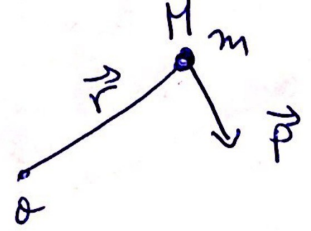
\includegraphics[width = \linewidth]{pic/conservationmomentangulair.png}
                        \end{minipage}
                    \end{center}
                \item Conservation de lenergie mecanique total 
                    \begin{itemize}
                        \item Theorem d energie cinetique \\
                            \begin{minipage}{0.49\linewidth}
                                $\Delta E_c = W$ , $W =\int\vv{F}d\vv{l}$
                            \end{minipage}
                            \begin{minipage}{0.39\linewidth}
                                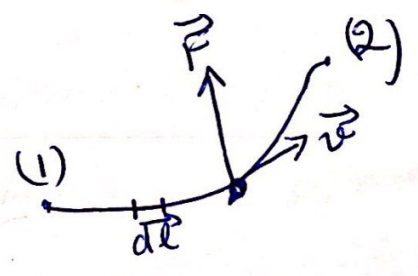
\includegraphics[width = \linewidth]{pic/theoremdenergiecinetique.png}
                            \end{minipage}
                        \item Forces conservatives \\ 
                            \begin{minipage}{0.49\linewidth}
                                si $W_{ACB} = W_{ADB} \implies$ les forces exterieur sont conservatives 
                            \end{minipage}
                            \begin{minipage}{0.39\linewidth}
                                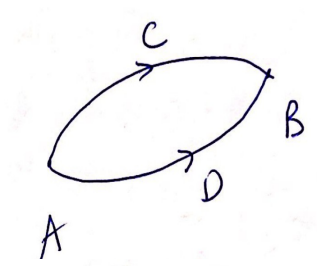
\includegraphics[width = \linewidth]{pic/frocesconservatives.png}
                            \end{minipage}
                        \item Une condition necessaire et suffisant pour que $W_{AB}$ soit independant du chemin est que $\vv{F}$ derive d un potentielle \\
                            $\vv{F} = -\vv{grad}(U)$ (U : energie potentielle)              
                    \end{itemize}        
            \end{itemize}
            \pagebreak
        \section{Contraintes et coordonees generalisees}
            Les contraintes du systeme introduisent des dependances entre les coordonee \\ 
            les contraintes sont par exemple des hypothese de rigidite , limitation de sont cadre d evolution $\ldots$ \\
            exemple :
            \begin{itemize}
                \item pendule simple \\
                \begin{minipage}{0.49\linewidth}
                    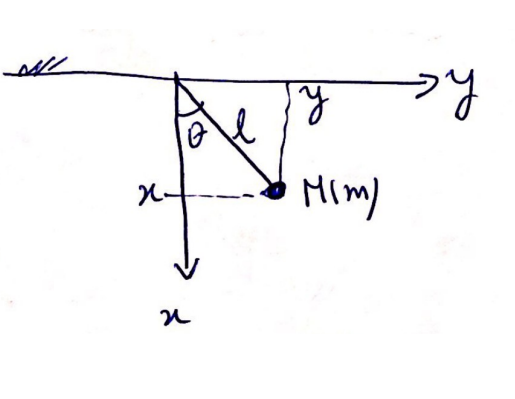
\includegraphics[width = \linewidth]{pic/pendulesimple.png}
                \end{minipage}
                \begin{minipage}{0.39\linewidth}
                    \boxed{x^2 + y^2 = l^2}
                \end{minipage}
                \item pendule simple \\
                \begin{minipage}{0.49\linewidth}
                    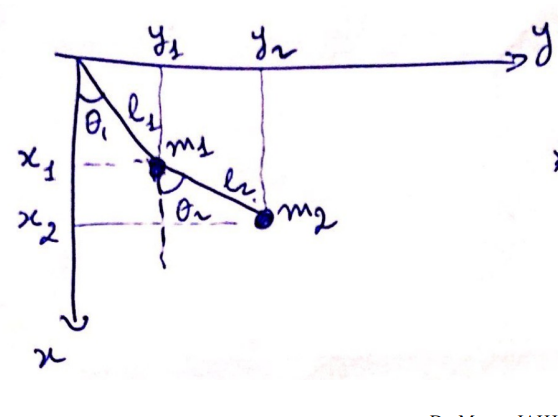
\includegraphics[width = \linewidth]{pic/penduledouble.png}
                \end{minipage}
                \begin{minipage}{0.39\linewidth}
                    \boxed{x_1^2 + y_1^2 = l_1^2} \\
                    \boxed{(x_2-x_1)^2 + (y_2 -y_1)^2 = l_2^2} 
                \end{minipage}
            \end{itemize}
            System de N particule 
            \begin{itemize}
                \item Aucun contraint (independante)$\implies$ 3N coordone (3N degree de liberte)
                \item K contrainte $\implies$ 3N -k coordonees independant 
            \end{itemize}
    \chapter{Formalise de lagrange}
        \section{Holonomic systeme }
            A system in which one can deduce the state of a system by knowing only information about the change of positions of the components of the system over time 
        \section{Calcule differentielle}
            Soit $f$ une fonctino de N variables $f=f(r_1 \ldots , r_N)$
            \begin{itemize}
                \item la differentielle totale de $f$ est : $df = \sum^N_{i=1}\frac{\partial f}{\partial r_i}dr_i$
                \item la derive de $f$ par rapport a lune de ses variable $(r_j)$ :
                 \[ \frac{df}{dr_j} = \sum^N_{i=1}\frac{\partial f}{\partial r_i}\frac{dr_i}{dr_j} \]
                 \item si tout les variable sont independant
                 \[ \frac{df}{dr_j} = \frac{\partial f}{\partial r_j} = \sum^N_{i=1}\frac{\partial f}{\partial r_i}\frac{dr_i}{dr_j} = \sum^N_{i=1}\frac{\partial f}{\partial r_i}\frac{\partial r_i}{\partial r_j} \]
            \end{itemize}
            \pagebreak
        \section{Equation generale de lagrange }
            On considere un system holonome de $N$ particule , $d$ degre du liberte , avex $\vv{F_\alpha}$ est la force appliquee sur la particule $\alpha$
            \subsection{lenergie cinetique est :}
                $T = \sum^N_{\alpha=1}T_\alpha =\sum^N_{\alpha=1}\frac{1}{2}m_\alpha\vv{\dot{r_\alpha}}^2 $ 
                \begin{itemize}
                    \item $\vv{r_\alpha} = \vv{r_\alpha}(q_1,q_2,q_3\ldots q_d ,t) $
                    \item $\alpha = 1,2,3 \ldots N$
                    \item $q_i$: coordone generalise 
                    \item $i=1,2,3\ldots d$
                    \item $\vv{\dot{r}} = \frac{d\vv{r_\alpha} }{dt}$
                \end{itemize}
                $T_\alpha = T_\alpha(\underbrace{q_1,q_2\ldots q_d}_{\text{position}} , \underbrace{\dot{q_1},\dot{q_2}\ldots\dot{q_d}}_{\text{vitess}} , \underbrace{t}_{\text{temp}}) $ \\
             \subsection{les forces generalise associe a $q_i$}
             \begin{center}
                \boxed{Q_i = \frac{d}{dt}\left( \frac{\partial T}{\partial \dot{q_i}} \right) - \frac{\partial T}{\partial q_i}}
             \end{center}
             \underline{Preuve :} \\ 
             \begin{itemize}
                \item on a :$dT = \sum^N_{\alpha =1} \frac{\partial T}{\partial \dot{r_\alpha}}d\dot{r_\alpha}$ (differentielle totale de $T$) 
                $\implies \frac{dT}{d\dot{q_i}} = \sum^N_{\alpha =1} \frac{\partial T}{\partial \dot{r_\alpha}}\frac{d\dot{r_\alpha}}{d\dot{q_i}}$ \\
                \item Puisque les variable sont independant alors :\\
                $ \frac{dT}{d\dot{q_i}}=\frac{\partial T}{\partial\dot{q_i}} = \sum^N_{\alpha =1} \frac{\partial T}{\partial \dot{r_\alpha}}\frac{\partial\dot{r_\alpha}}{\partial\dot{q_i}}$ 
                $\implies \frac{\partial T}{\partial \dot{q_i}}=\frac{\partial}{\partial \dot{q_i}}(\sum^N_{\alpha =1} \frac{1}{2}m_\alpha(\vv{\dot{r_\alpha}})^2)= \frac{1}{2}(\sum^N_{\alpha =1} m_\alpha \frac{\partial}{\partial\dot{q_i}}(\vv{\dot{r_\alpha}})^2)$
                \\ $= \frac{1}{2}\times 2 \sum^N_{\alpha =1} m_\alpha \vv{\dot{r_\alpha}}\frac{\partial \vv{\dot{r_\alpha}}}{\partial\dot{q_i}} \implies$ \boxed{\frac{\partial T}{\partial \dot{q_i}} = \sum^N_{\alpha =1} m_\alpha\vv{\dot{r_\alpha}}\frac{\partial\vv{\dot{r_\alpha}}}{\partial\dot{q_i}}}\\
                \pagebreak
                \item Chercher $\vv{\dot{r_\alpha}}$ , ona :
                \begin{itemize}
                    \item $\vv{r_\alpha} = \vv{r_\alpha} (q_1,q_2\ldots q_d , t) $
                    \item $\vv{r_\alpha} = \frac{d((\vv{r_\alpha}))}{dt}$
                \end{itemize}
                $d\vv{r_\alpha} = \frac{\partial\vv{r_\alpha}}{\partial q_1}dq_1+\frac{\partial\vv{r_\alpha}}{\partial q_2}dq_2 + \ldots +\frac{\partial\vv{r_\alpha}}{\partial q_d}dq_d+\frac{\partial\vv{r_\alpha}}{\partial t}dt$ \\
                $\frac{d\vv{r_\alpha}}{dt} =\vv{\dot{r_\alpha}}= \frac{\partial\vv{r_\alpha}}{\partial q_1}\frac{dq_1}{dt}+\frac{\partial\vv{r_\alpha}}{\partial q_2}\frac{dq_2}{dt} + \ldots +\frac{\partial\vv{r_\alpha}}{\partial q_d}\frac{dq_d}{dt}+\frac{\partial\vv{r_\alpha}}{\partial t}$ \\
                $\frac{d\vv{r_\alpha}}{dt} =\vv{\dot{r_\alpha}}= \frac{\partial\vv{r_\alpha}}{\partial q_1}\frac{\partial q_1}{\partial t}+\frac{\partial\vv{r_\alpha}}{\partial q_2}\frac{\partial q_2}{\partial t} + \ldots +\frac{\partial\vv{r_\alpha}}{\partial q_d}\frac{\partial q_d}{\partial t}+\frac{\partial\vv{r_\alpha}}{\partial t}$ \\
                \begin{center}
                    \boxed{\vv{\dot{r_\alpha}}= \sum^d_{i =1}\frac{\partial\vv{r_\alpha}}{\partial q_i}\dot{q_i}+\frac{\partial \vv{r_\alpha}}{\partial t}  } avec $\alpha = 1,2\ldots N$
                \end{center}
                \item demontrer que $\frac{\partial\vv{\dot{r_\alpha}}}{\partial\dot{q_i}} = \frac{\partial\vv{r_\alpha}}{\partial q_i}$ \\ 
                $\vv{\dot{r_\alpha}} =\sum^d_{i =1} \frac{\partial\vv{r_\alpha}}{\partial q_i}\dot{q_i} + \frac{\partial r_\alpha}{\partial t} = \frac{\partial \vv{r_\alpha}}{\partial q_1}\dot{q_1} + \ldots+ \frac{\partial \vv{r_\alpha}}{\partial q_i}\dot{q_i} + \ldots + \frac{\partial \vv{r_\alpha}}{\partial q_d}\dot{q_d} +\frac{\partial \vv{r_\alpha}}{\partial t}(q_i,t)$ \\
                $\frac{\partial}{\partial \dot{q}}\left( \frac{\partial\vv{r}}{\partial t} \right) = 0$ car $\frac{\partial\vv{r}}{\partial t} = \frac{\partial \vv{r}}{\partial t}(q_i,t)$ \\
                $\frac{\partial \vv{\dot{r_\alpha}}}{\partial\dot{q_i}} = 0 +0 +0 \ldots + \frac{\partial \vv{r_\alpha }}{\partial q_i}\frac{\partial \dot{q_i}}{\partial \dot{q_i}} + \ldots + 0$ \\
                $=\frac{\partial\vv{r_\alpha}}{\partial q_i} = \frac{\partial\vv{r_\alpha}}{\partial q_i} \implies$\boxed{\frac{\partial\vv{\dot{r_\alpha}}}{\partial\dot{q_i}} = \frac{\partial\vv{r_\alpha}}{\partial q_i}} \\
                \item alors $\frac{\partial T}{\partial \dot{q_i}} =\sum^N_{\alpha =1}m_\alpha \vv{\dot{r_\alpha}}\frac{\partial \vv{\dot{r_\alpha}}}{\partial \dot{q_i}} \implies $ \boxed{\frac{\partial T}{\partial \dot{q_i}} =\sum^N_{\alpha =1}m_\alpha \vv{\dot{r_\alpha}}\frac{\partial \vv{r_\alpha}}{\partial q_i}}\\
                \item Calcule de $\frac{d}{dt}\left( \frac{\partial T}{\partial \dot{q_i}} \right)$ \\
                \begin{itemize}
                    \item $ \frac{d}{dt}\left( \frac{\partial T}{\partial \dot{q_i}} \right) =\frac{d}{dt}\left( \sum^N_{\alpha = 1}m_\alpha\vv{\dot{r_\alpha}}\frac{\partial \vv{r_\alpha}}{\partial q_i} \right) = \sum^N_{\alpha = 1}m_\alpha \vv{\ddot{r_\alpha}} \frac{\partial \vv{r_\alpha}}{\partial q_i} + \sum^N_{\alpha = 1}m_\alpha\vv{\dot{r_\alpha}}\underbrace{\frac{d}{dt}\left( \frac{\partial \vv{r_\alpha}}{\partial q_i} \right)}$ \\
                    \item Calcule de $\frac{d}{dt}\left( \frac{\partial \vv{r_\alpha}}{\partial q_i} \right)$ \\ 
                        $d\left( \frac{\partial \vv{r_\alpha}}{\partial q_i} \right) = \sum^d_{i=1}\frac{\partial}{\partial q_i} \left( \frac{\partial \vv{r_\alpha}}{\partial q_i} \right)dq_i + \frac{\partial}{\partial t}\left( \frac{\partial \vv{r_\alpha}}{\partial q_i} \right)dt$\\
                        $\frac{d}{dt}\left( \frac{\partial \vv{r_\alpha}}{\partial q_i} \right) = \sum^d_{i=1}\frac{\partial}{\partial q_i} \left( \frac{\partial \vv{r_\alpha}}{\partial q_i} \right)\dot{q_i} + \frac{\partial}{\partial t}\left( \frac{\partial \vv{r_\alpha}}{\partial q_i} \right) \implies \frac{d}{dt}\left( \frac{\partial \vv{r_\alpha}}{\partial q_i} \right) = \sum^d_{i=1}\frac{\partial}{\partial q_i} \left( \frac{\partial \vv{r_\alpha}}{\partial q_i} \right)\dot{q_i} + \frac{\partial}{\partial q_i}\left( \frac{\partial \vv{r_\alpha}}{\partial t} \right)$\\
                        $\frac{d}{dt}\left( \frac{\partial \vv{r_\alpha}}{\partial q_i} \right) = \frac{\partial}{\partial q_i} \left( \sum^d_{i=1} \frac{\partial\vv{r_\alpha}}{\partial q_i} \dot{q_i} + \frac{\partial}{\partial t}\vv{r_\alpha} \right) = \frac{\partial}{\partial q_i}\vv{\dot{r_\alpha}} = \frac{\partial}{\partial q_i}\frac{d}{dt}(\vv{r_\alpha}) \implies $ \boxed{\frac{d}{dt}\left( \frac{\partial \vv{r_\alpha}}{\partial q_i} \right)= \frac{\partial}{\partial q_i}\vv{\dot{r_\alpha}} } \\
                    \item Verifier que $\sum^N_{\alpha = 1}m_\alpha \vv{\ddot{r_\alpha}} \frac{\partial \vv{r_\alpha}}{\partial q_i} = \frac{\partial T}{\partial q_i} $\\
                        on a $T = \sum^N_{\alpha =1 }m_\alpha\vv{\dot{r_\alpha}}^2 $ 
                        $\implies \frac{\partial T}{\partial q_i} =  \sum^N_{\alpha =1 }m_\alpha\frac{\partial}{\partial q_i}(\vv{\dot{r_\alpha}})^2 \implies$
                        \boxed{\frac{\partial T}{\partial q_i}= \sum^N_{\alpha =1 }m_\alpha\vv{\dot{r_\alpha}}\frac{\partial \vv{\dot{r_\alpha}}}{\partial q_i}}
                \end{itemize}
                alors \begin{center}
                    \boxed{\frac{d}{dt}\left( \frac{\partial T}{\partial \dot{q_i}} \right) =\frac{\partial T}{\partial q_i} + \sum^N_{\alpha = 1}m_\alpha\vv{\dot{r_\alpha}}\frac{\partial}{\partial q_i}\vv{\dot{r_\alpha}} }
                \end{center}
                \item on utilise la loi de Newton : $ \vv{F_\alpha} = m_\alpha\vv{\ddot{r_\alpha}} \implies  \frac{d}{dt}\left( \frac{\partial T}{\partial \dot{q_i}} \right) =\frac{\partial T}{\partial q_i} + \sum^N_{\alpha = 1}\vv{F_\alpha}\frac{\partial\vv{\dot{r_\alpha}}}{\partial q_i}$  \\
                avec $\sum^N_{\alpha = 1}\vv{F_\alpha}\frac{\partial\vv{\dot{r_\alpha}}}{\partial q_i} = Q_i$
                \begin{center}
                    \boxed{Q_i = \frac{d}{dt}\left( \frac{\partial T}{\partial \dot{q_i}} \right) - \frac{\partial T}{\partial q_i}}
                \end{center}
             \end{itemize}
        \section{Formalisme de lagrange : cas d un system conservatif}
             \begin{itemize}
                \item Si les forces $\vv{F_\alpha}$ sont conservatif , On suppose que toutes les forces agissant sur ce system derivent d'ume mem energie potentielle $U$ \\
                    avex $U$ depend de position $U = U(\vv{r_1}, \vv{r_2}\ldots , \vv{r_N})$ et $\vv{F_\alpha}=-\vv{grad}U$ \\
                    Donc , on a \boxed{\sum^N_{\alpha =1 }\vv{F_\alpha}d\vv{r_\alpha}=-dU}
                \item On a l equation de lagrange $\frac{d}{dt}\left( \frac{\partial T}{\partial \dot{q_i}} \right) - \frac{\partial T}{\partial q_i} = \sum^N_{\alpha = 1}\vv{F_\alpha}\frac{\partial\vv{\dot{r_\alpha}}}{\partial q_i} = Q_i$ \\
                    avec $Q_i =\sum^N_{\alpha = 1}\vv{F_\alpha}\frac{\partial\vv{\dot{r_\alpha}}}{\partial q_i} = \frac{-dU}{dq_i}\implies $ \boxed{Q_i =\frac{-\partial U}{\partial q_i}}(si les forces sont conservatives)
                \item L'equation devien $\frac{d}{dt}\left( \frac{\partial T}{\partial \dot{q_i}} \right) - \frac{\partial T}{\partial q_i} = \frac{-\partial U}{\partial q_i} \implies \frac{d}{dt}\left( \frac{\partial T}{\partial \dot{q_i}} \right) = \frac{-\partial}{\partial q_i}(T-U) =0$ 
                \item U depend seulment du position alors $\frac{\partial T}{\partial \dot{q_i}} = \frac{\partial}{\partial \dot{q_i}}(T-U)$ \\
                    l equation devien $\frac{d}{dt}\left( \frac{\partial}{\partial \dot{q_i}}(T-U) \right) - \frac{\partial}{\partial q_i} (T-U) =0$
                \item On introdui la fonction de lagrange (lagrangien) \\
                    \begin{center}
                        \boxed{L(qi,\dot{q_i},t) = T- U } \\
                        $T$ depend de vitess $\dot{q_i}$ et $U$ depend de position $q_i$
                    \end{center}
                \item L equation devien \\
                    \begin{center}
                        Equation Euler-lagrange : \boxed{\frac{d}{dt}\left( \frac{\partial L}{\partial \dot{q_i}} \right) - \frac{\partial L}{\partial q_i} =0}
                    \end{center}
            \end{itemize}
\end{document}